% !TEX TS-program = pdflatex
% !TEX encoding = UTF-8 Unicode

% This is a simple template for a LaTeX document using the "article" class.
% See "book", "report", "letter" for other types of document.

\documentclass[20pt]{article} % use larger type; default would be 10pt

\usepackage[utf8]{inputenc} % set input encoding (not needed with XeLaTeX)

%%% Examples of Article customizations
% These packages are optional, depending whether you want the features they provide.
% See the LaTeX Companion or other references for full information.

%%% PAGE DIMENSIONS
\usepackage{geometry} % to change the page dimensions
\geometry{a4paper} % or letterpaper (US) or a5paper or....
% \geometry{margin=2in} % for example, change the margins to 2 inches all round
% \geometry{landscape} % set up the page for landscape
%   read geometry.pdf for detailed page layout information

\usepackage{graphicx} % support the \includegraphics command and options

% \usepackage[parfill]{parskip} % Activate to begin paragraphs with an empty line rather than an indent

%%% PACKAGES
\usepackage{booktabs} % for much better looking tables
\usepackage{array} % for better arrays (eg matrices) in maths
\usepackage{paralist} % very flexible & customisable lists (eg. enumerate/itemize, etc.)
\usepackage{verbatim} % adds environment for commenting out blocks of text & for better verbatim
%\usepackage{subfig} % make it possible to include more than one captioned figure/table in a single float
\usepackage{mathtools}
\usepackage{graphicx} % supports images in latex
% These packages are all incorporated in the memoir class to one degree or another...

\usepackage{graphicx}
\usepackage{subcaption}

%%% Other stuff
\DeclarePairedDelimiter\ceil{\lceil}{\rceil}
\DeclarePairedDelimiter\floor{\lfloor}{\rfloor}

%%% HEADERS & FOOTERS
\usepackage{fancyhdr} % This should be set AFTER setting up the page geometry
\pagestyle{fancy} % options: empty , plain , fancy
\renewcommand{\headrulewidth}{0pt} % customise the layout...
\lhead{}\chead{}\rhead{}
\lfoot{}\cfoot{\thepage}\rfoot{}

%%% SECTION TITLE APPEARANCE
\usepackage{sectsty}
\allsectionsfont{\sffamily\mdseries\upshape} % (See the fntguide.pdf for font help)
% (This matches ConTeXt defaults)

%%% ToC (table of contents) APPEARANCE
\usepackage[nottoc,notlof,notlot]{tocbibind} % Put the bibliography in the ToC
\usepackage[titles,subfigure]{tocloft} % Alter the style of the Table of Contents
\renewcommand{\cftsecfont}{\rmfamily\mdseries\upshape}
\renewcommand{\cftsecpagefont}{\rmfamily\mdseries\upshape} % No bold!

%%% graphics path


%%% END Article customizations

%%% nice things to keep around
%\begin{figure}[!htbp]
%  	\centering
%   	\begin{subfigure}[p]{0.5\linewidth}
%    	\includegraphics[width=\linewidth]{}
%   	\end{subfigure}
%\end{figure} 

% \noindent\rule{2cm}{0.4pt} 
%%% puts a small horizontal line

% \mathcal{O} 
%%% big O notation

% \begin{table}
% \caption{Forward slash.}
% \[\begin{array}{c|ccccc} 
% abc/def & 1 & 2 & 3 & 4 & 5\\
% \hline
% 1 & a & b & c & d & e\\
% 2 & f & g & h & i & j\\
% 3 & k & l & m & n & o\\
% \end{array}\]
% \end{table}

%%% The "real" document content comes below...

\title{Formal Languages Homework 6}
\author{Liam Dillingham}
%\date{} % Activate to display a given date or no date (if empty),
         % otherwise the current date is printed 

\begin{document}
\maketitle

\section{Problem 4.1.1 and 4.1.2}
Provide the CFG for the following languages: 
\subsection{b). The set of strings of balanced parentheses. These are the strings of characters $"("$ and $")"$ that can appear in a well-formed arithmetic expression.}
$S \rightarrow (S) \mid SS \mid \epsilon$.\\
$ V = \{ S \}$. \\ 
$T = \{ \ "(", \ ")" \ \}$. (The quotations are only to make reading easier).

\subsection{d). $\{0^{n}1^{m}2^{n} \mid n$ and $m$ are abitrary integers $\}$.}
$V = \{ S, A \}$. \\
$T = \{0,1,2\}$.\\
 \begin{table}[!htbp]
 \[\begin{array}{ccc} 
&  \\
 S & \rightarrow & 0S2 \mid 0A2 \mid A \mid \epsilon\\
 A & \rightarrow & 1 \mid \epsilon \\
 \end{array}\]
 \end{table}
\subsection{f). $\{0^{n}1^{2n} \mid n \geq 1\}$}
$V = \{S, A\}$ \\
$T = \{0, 1\}$\\
 \begin{table}[!htbp]
 \[\begin{array}{ccc} 
&  \\
 S & \rightarrow & 0S11 \mid 0A11 \\
 A & \rightarrow & \epsilon \\
 \end{array}\]
 \end{table}
\subsection{h). The set of strings of the form $w1^{n}$, where $w$ is a string of 0's and 1's of length $n$.}
$V = \{S,a\}$\\
$T = \{0,1\}$\\
 \begin{table}[!htbp]
 \[\begin{array}{ccc} 
&  \\
 S & \rightarrow & AS1 \mid \epsilon \\
 A & \rightarrow & 0 \mid 1 \\
 \end{array}\]
 \end{table}
\section{Problem 5.1.2}
The following grammar generates the language of regular expression $0^{*}1(0+1)^{*}$. 
 \begin{table}[!htbp]
 \[\begin{array}{ccc} 
&  \\
 S & \rightarrow & A1B\\
 A & \rightarrow & 0A \mid \epsilon \\
 B & \rightarrow  & 0B \mid 1B \mid \epsilon \\
 \end{array}\]
 \end{table} \\
Give leftmost and rightmost derivations of the following strings:
\subsection{a). 00101.}
Leftmost: \\ 
$S\Rightarrow A1B \Rightarrow 0A1B \Rightarrow 00A1B \Rightarrow 00\epsilon1B \Rightarrow 001B \Rightarrow 0010B \Rightarrow 00101B \Rightarrow 00101\epsilon \Rightarrow 00101.$ \\
Rightmost: \\
$S\Rightarrow A1B \Rightarrow A10B \Rightarrow A101B \Rightarrow A101\epsilon \Rightarrow A101 \Rightarrow 0A101 \Rightarrow 00A101 \Rightarrow 00\epsilon101 \Rightarrow00101$.
\subsection{b). 1001.}
Leftmost:\\
$S\Rightarrow A1B \Rightarrow \epsilon1B \Rightarrow 10B \Rightarrow 100B \Rightarrow 1001B \Rightarrow 1001\epsilon \Rightarrow 1001$. \\
Rightmost:\\
$S \Rightarrow A1B \Rightarrow A10B \Rightarrow A100B \Rightarrow A1001B \Rightarrow A1001\epsilon \Rightarrow \epsilon1001 \Rightarrow 1001$.
\subsection{c). 00011.}
Leftmost:\\
$S \Rightarrow A1B \Rightarrow 0A1B \Rightarrow 00A1B \Rightarrow 000A1B \Rightarrow 000\epsilon1B \Rightarrow 00011B \Rightarrow 00011\epsilon \Rightarrow 00011$. \\
Rightmost:\\
$S \Rightarrow A1B \Rightarrow A11B \Rightarrow A11\epsilon \Rightarrow 0A11 \Rightarrow 00A11 \Rightarrow 000A11 \Rightarrow 000\epsilon11 \Rightarrow 00011$.

\newpage
\section{Problem 5.2.1}
For the grammar and each of the strings in Exercise 5.1.2, give parse trees. 
\subsection{a). 00101.}
\begin{figure}[!htbp]
  	\centering
   	\begin{subfigure}[p]{0.5\linewidth}
    	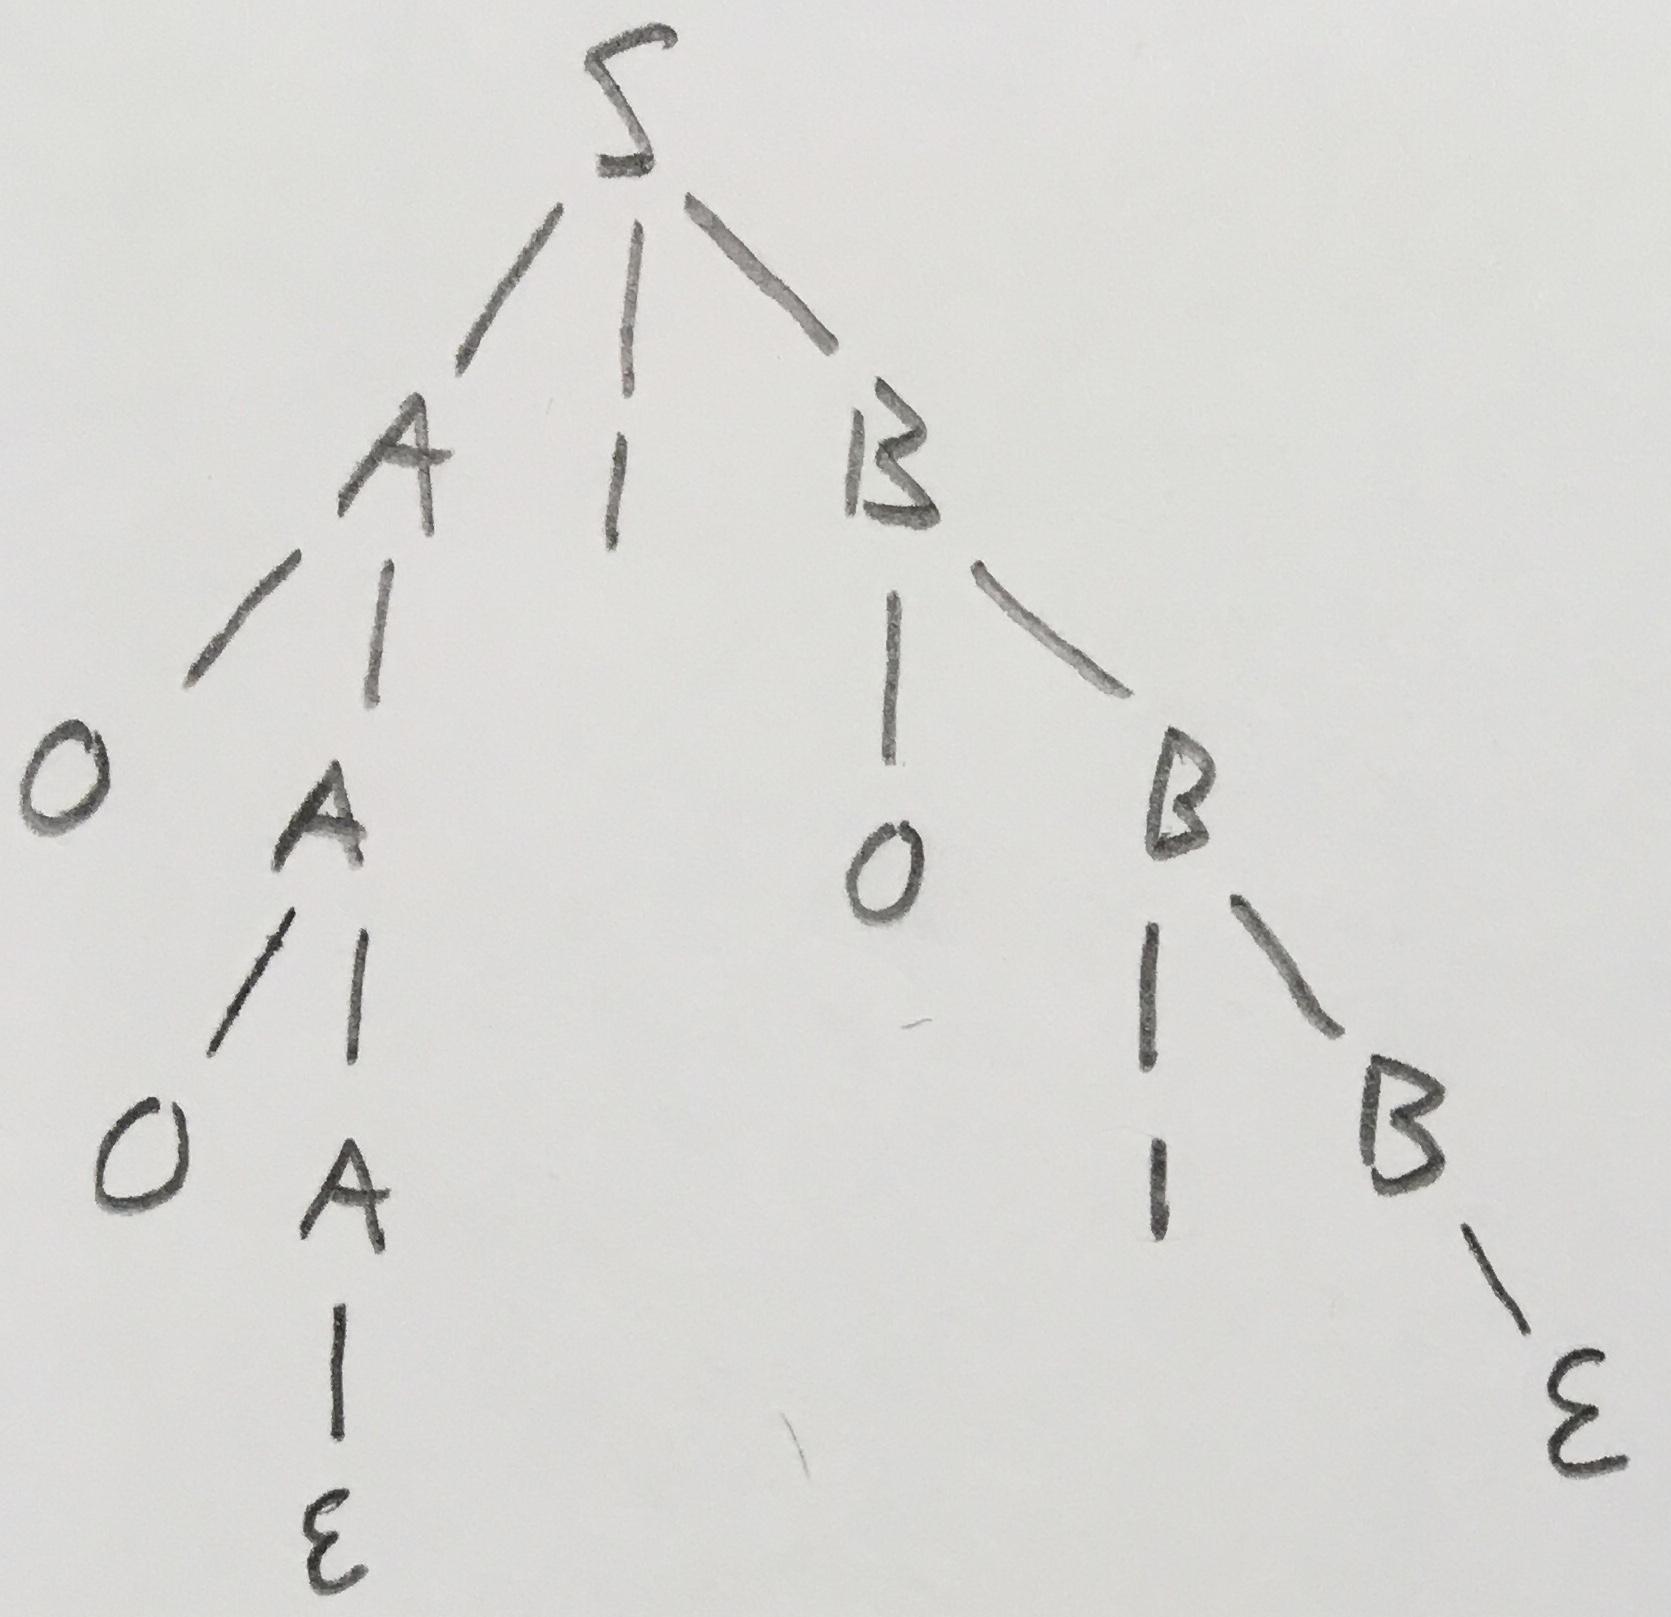
\includegraphics[width=\linewidth]{./figures/h6-1.jpg}
   	\end{subfigure}
\end{figure} 
\subsection{b). 1001.}
\begin{figure}[!htbp]
  	\centering
   	\begin{subfigure}[p]{0.5\linewidth}
    	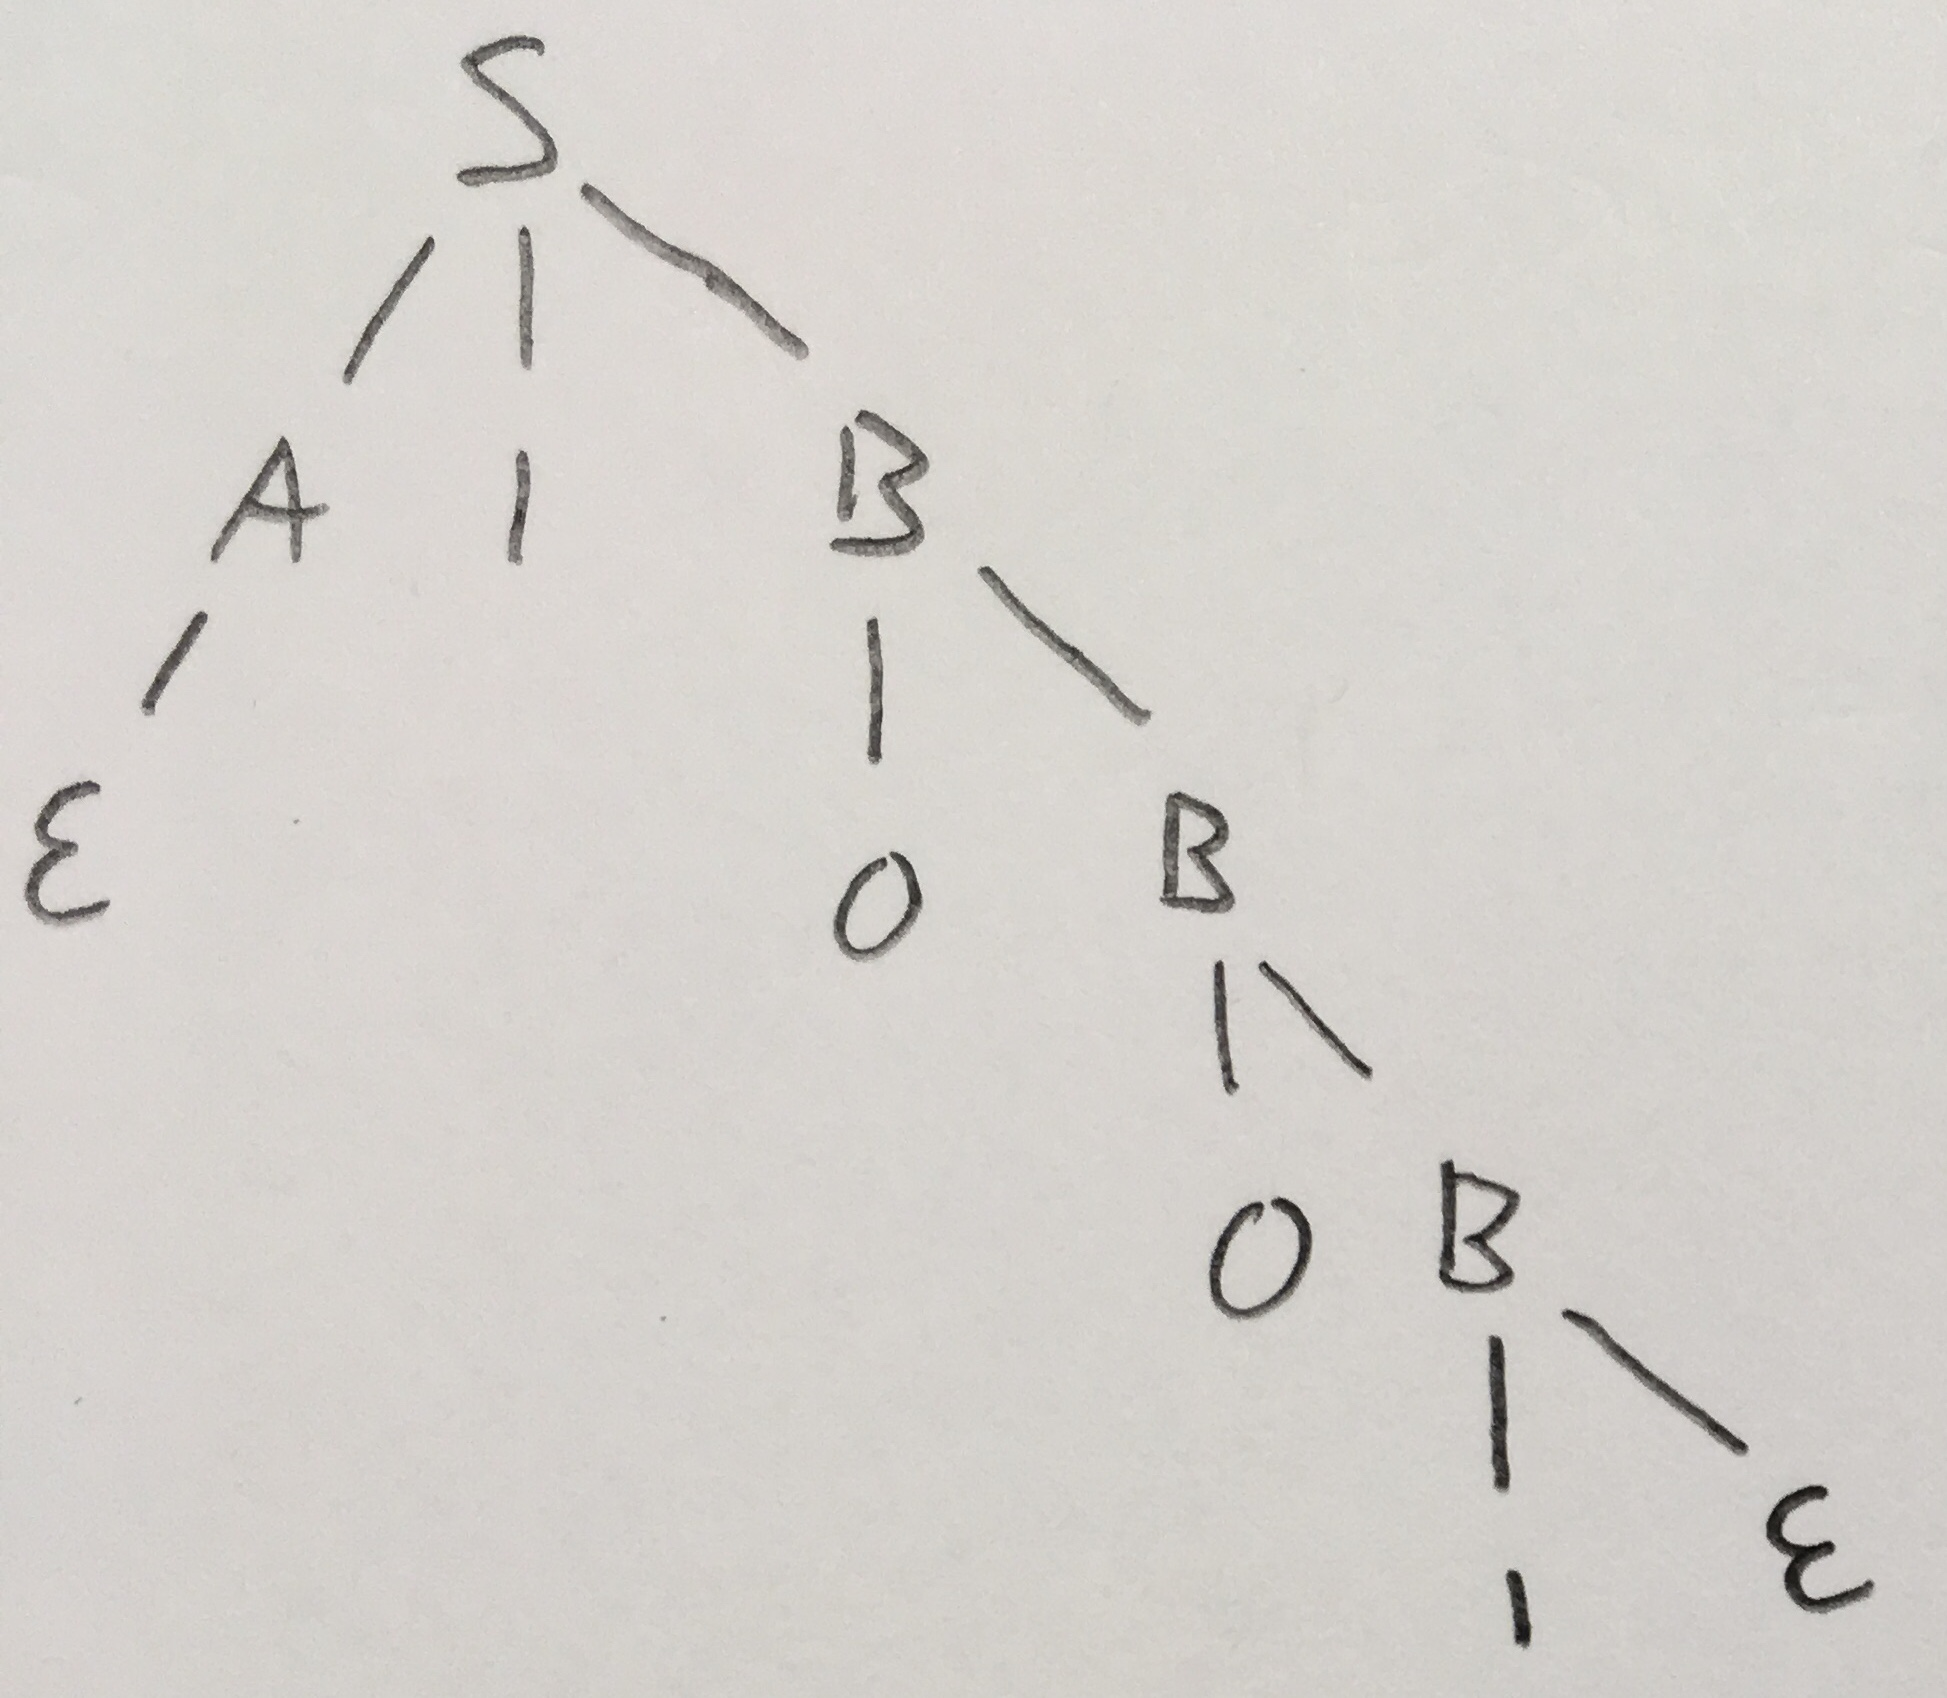
\includegraphics[width=\linewidth]{./figures/h6-2.jpg}
   	\end{subfigure}
\end{figure} 
\newpage
\subsection{c). 00011.}
\begin{figure}[!htbp]
  	\centering
   	\begin{subfigure}[p]{0.4\linewidth}
    	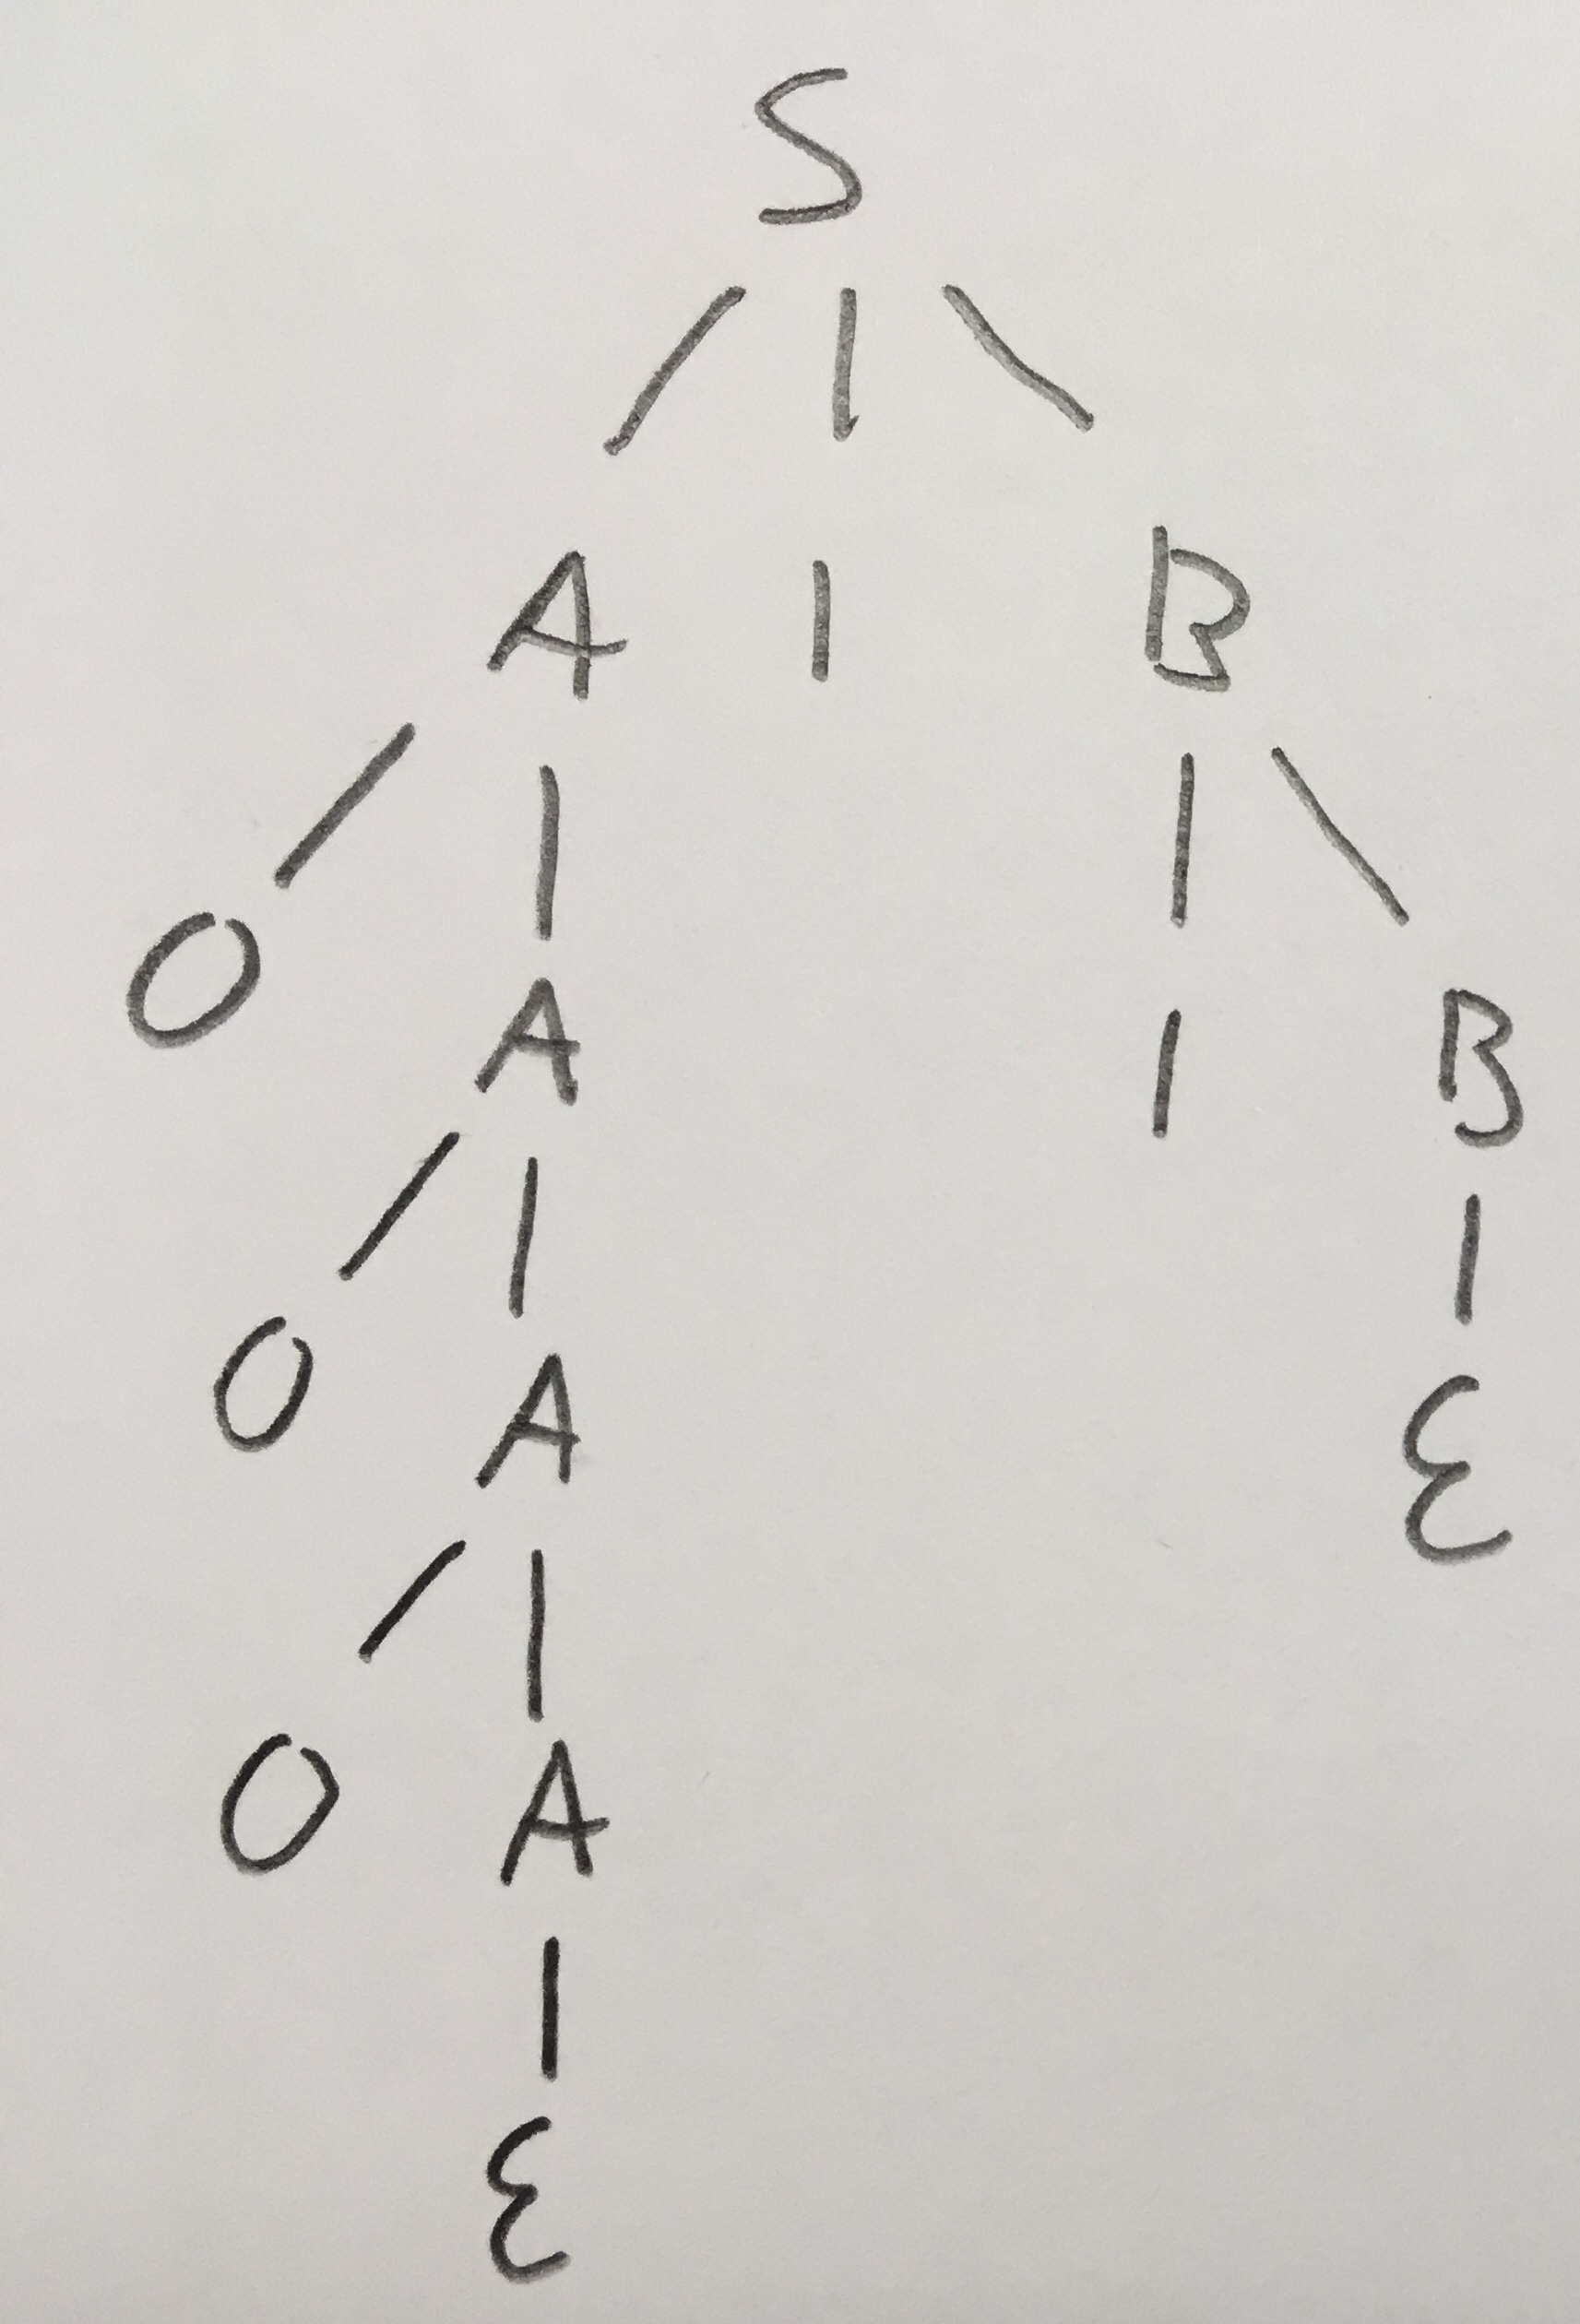
\includegraphics[width=\linewidth]{./figures/h6-3.jpg}
   	\end{subfigure}
\end{figure} 

\section{Problem 5.4.5}
This question concerns the grammar from Exercise 5.1.2
\subsection{a). Show that this grammar is unambiguous}
\textit{Base case}: The shortest string we can make. since $S \rightarrow A1B$, and it is possible such that $A \rightarrow \epsilon$ and $ B \rightarrow \epsilon$, then the smallest $w$ is $|w| = 1$.  And there is only one derivation for this. \\
\textit{Inductive Hypothesis}:  Assume that for all $w \in \{0,1\}^{*}$, with $|w| = n$, where $n \geq 1$, $w$ has at most 1 left-most derivation from $S,A,B$. \\
\textit{Inductive Step}: Show that the hypothesis holds for $w$, $|w| = n+1$, $n \geq 1$. \\
\textit{Case 1}: Show that for each $A \Rightarrow^{*} w$, there is aunique LM derivation $A \Rightarrow_{LM}^{*} w$. \\
\textit{Proof}: Since $A \Rightarrow_{LM}^{*} w$, replace $A$ with string $y$. Then $|y| \leq n$ because $|w| = n+1$. Note that because $|y| = n$, that $y$ has a unique leftmost derivation from $A$.  Thus $A \Rightarrow_{LM}^{*} 0y = w$.  The same argument follows for $B$.  Since the hypothesis holds true for both $A$ and $B$, then certainly it holds true for $S$, since $S \rightarrow A1B$.  Thus the grammar is unambiguous.

\newpage
\subsection{b). Find a grammar for the same language that \textit{is} ambiguous, and demonstrate its ambiguity}
Let G:
 \begin{table}[!htbp]
 \[\begin{array}{ccc} 
&  \\
 S & \rightarrow & A1B \\
 A & \rightarrow & 0A \mid 00A \mid \epsilon \\
 B & \rightarrow & bBc \mid \epsilon
 \end{array}\]
 \end{table}

Suppose we want to find the derivation for $0001$. We have two derivations:\\
$ S \Rightarrow A1B \Rightarrow 0A1B \Rightarrow 00A1B \Rightarrow 000A1B \Rightarrow 000\epsilon 1B \Rightarrow 0001B \Rightarrow 0001\epsilon \Rightarrow 0001$. \\
$ S \Rightarrow A1B \Rightarrow 00A1B \Rightarrow 000A1B \Rightarrow 000\epsilon 1B \Rightarrow 0001\epsilon \Rightarrow 0001$. \\

Thus the grammar is ambiguous

\noindent\rule{15cm}{0.4pt} \\
Additional Exercises
\section{Problem 1}
Design a regular grammar without using a variable goes to $\epsilon$ rule $(A \rightarrow \epsilon)$ for the set of binary strings beginning with 1, ending with 0, and having even number of 0's and even number of 1's.
 \noindent\rule{2cm}{0.4pt} \\

 \begin{table}[!htbp]
 \[\begin{array}{ccc} 
&  \\
 S & \rightarrow & 1A0 \\
 A & \rightarrow &  1 \\
 \end{array}\]
 \end{table}

\section{Problem 2}
Design context-free grammars for the following languages
\subsection{1). $L = \{ a^{n}b^{m}c^{2n+m} \mid n,m > 0\}$ where $\Sigma = \{a,b,c\}$}
 \begin{table}[!htbp]
 \[\begin{array}{ccc} 
&  \\
 S & \rightarrow & aAbccc \\
 A & \rightarrow & aABcc \mid \epsilon \\
 B & \rightarrow & bBc \mid \epsilon
 \end{array}\]
 \end{table}
\subsection{2). $L = \{a^{n}b^{m}c^{i} \mid m > n + i$ and $m,n,i \geq 0\}$, where $\Sigma = \{a,b,c\}$}
 \begin{table}[!htbp]
 \[\begin{array}{ccc} 
&  \\
 S & \rightarrow & aAbbBbCc \\
 A & \rightarrow & aAb \mid \epsilon \\
 B & \rightarrow & bBb \mid \epsilon \\
 C & \rightarrow & bCc \mid \epsilon 
 \end{array}\]
 \end{table}
\subsection{3). $L = \{a^{m}b^{n} \mid 0 \leq n \leq m \leq 3n\}$, where $\Sigma = \{a,b\}$}
 \begin{table}[!htbp]
 \[\begin{array}{ccc} 
&  \\
 S & \rightarrow & aaAb \\
 A & \rightarrow & aaAb \mid \epsilon 
 \end{array}\]
 \end{table}
\section{Problem 3}
Let $G$ be the grammar
 \begin{table}[!htbp]
 \[\begin{array}{ccc} 
&  \\
 S & \rightarrow & ASB \mid ab \mid SS\\
 A & \rightarrow & aA \mid \epsilon \\
 B & \rightarrow  & bB \mid \epsilon \\
 \end{array}\]
 \end{table}
\subsection{1). Give a leftmost derivation of aaabb}
$S \Rightarrow ASB \Rightarrow aASB \Rightarrow aaASB \Rightarrow aa\epsilon SB \Rightarrow aaabB \Rightarrow aaabbB \Rightarrow aaabb\epsilon \Rightarrow aaabb$
\subsection{2). Give a rightmost derivation of aaabb}
$S \Rightarrow ASB \Rightarrow ASbB \Rightarrow ASb\epsilon \Rightarrow Aabb \Rightarrow aAabb \Rightarrow aaAabb \Rightarrow aa\epsilon abb \Rightarrow aaabbb$
\subsection{3). Show that G is ambiguous}
We can show that G is ambiguous by showing that there are two distinct leftmost derivations for a given string (ex. $aaabb$).  \\



$S \Rightarrow ASB \Rightarrow aASB \Rightarrow aaASB \Rightarrow aa\epsilon SB \Rightarrow aaabB \Rightarrow aaabbB \Rightarrow aaabb\epsilon \Rightarrow aaabb$. \\


$S \Rightarrow ASB \Rightarrow aASB \Rightarrow aaASB \Rightarrow aa\epsilon SB \Rightarrow aaASBB \Rightarrow aa\epsilon SBB \Rightarrow aaabBB \Rightarrow aaabbBB \Rightarrow aaabb\epsilon \epsilon \Rightarrow aaabb.$ \\

Thus G is ambiguous

\subsection{4). Construct an unambiguous grammar equivalent to G}.
 \begin{table}[!htbp]
 \[\begin{array}{ccc} 
&  \\
 S & \rightarrow & AB \\
 A & \rightarrow & aA \mid \epsilon \\
 B & \rightarrow  & bB \mid \epsilon \\
 \end{array}\]
 \end{table}
\end{document}






































